\chapterimage{tabl_cont3.pdf} % Chapter heading image

\chapter{Qlik}
\section{Introduzione}
\textbf{Qlik} è una società statunitense di software, con sede in Pennsylvania, fondata nel 1993 a Lund, in Svezia. La compagnia, il cui logo è mostrato alla Figura \ref{fig:QlikLogo}, è nota per aver sviluppato una piattaforma avanzata di Business Intelligence, che consente alle aziende di trasformare i propri dati in informazioni strategiche attraverso tecniche di analisi visiva e interattiva. Utilizzando il motore associativo, Qlik permette agli utenti di esplorare i dati in modo dinamico, creando visualizzazioni intuitive volte a semplifiicare il processo decisionale. La capacità di integrare e visualizzare grandi volumi di dati provenienti da diverse fonti in tempo reale rappresenta uno degli aspetti distintivi della piattaforma, rendendo Qlik uno strumento potente per analisi complesse e reporting.

\begin{figure}[h!]
    \centering
    
\includegraphics[width=0.35\linewidth]{capitolo_1/img1/QlikLogo.pdf}
    \caption{Qlik - Logo}
    \label{fig:QlikLogo}
\end{figure}

Qlik offre diverse applicazioni e strumenti, tra cui Qlik Sense e QlikView, che rispondono a diverse esigenze di business e di analisi dei dati. \textbf{Qlik Sense} è una piattaforma di Business Intelligence self-service progettata per offrire una creazione di report e dashboard personalizzati, con una forte enfasi sull'interattività e sulla visualizzazione dei dati. Grazie alla sua interfaccia intuitiva, Qlik Sense consente agli utenti di esplorare i dati autonomamente, creando visualizzazioni dinamiche e analisi ad hoc senza necessitare di competenze tecniche avanzate. Inoltre, Qlik Sense si distingue per la sua capacità di adattarsi facilmente a diverse fonti di dati, offrendo funzionalità di drag-and-drop, capacità di collaborazione e scalabilità in ambienti aziendali complessi. È particolarmente adatto a organizzazioni che desiderano democratizzare l'accesso ai dati, dando a tutti i livelli aziendali la possibilità di fare analisi e prendere decisioni basate sui dati in tempo reale.

D'altra parte, \textbf{QlikView} è una soluzione di BI più tradizionale e predefinita, progettata per rispondere a esigenze aziendali strutturate e complesse. Mentre Qlik Sense è più orientato all’autonomia dell'utente, QlikView richiede una configurazione più tecnica e un'implementazione più centralizzata. È ideale per le aziende che necessitano di soluzioni di reporting più fisse e predeterminate, dove l'analisi è spesso guidata da requisiti specifici di business e processi consolidati. QlikView consente la creazione di applicazioni di analisi altamente personalizzate e report standardizzati, spesso progettati da sviluppatori IT o team di BI, per soddisfare le necessità analitiche in modo scalabile e sicuro.

La versatilità della piattaforma consente di rispondere in modo rapido alle necessità aziendali, migliorando la capacità di prendere decisioni informate e basate su dati concreti. In tale contesto, l'adozione di Qlik consente alle organizzazioni di ottimizzare i propri processi aziendali, ottenere insight più approfonditi e supportare strategie orientate alla crescita.


\subsection{Caricamento e preparazione del dataset}
Il processo di caricamento dei dati su Qlik è una fase cruciale che consente di importare e integrare dati provenienti da diverse fonti e in vari formati, tra cui database relazionali come \textit{SQL Server}, \textit{Oracle} e \textit{MySQL}, file flat (\textit{CSV}, \textit{Excel}), applicazioni cloud come \textit{Google Analytics} e \textit{Salesforce}, nonché altre fonti esterne.
A differenza di altri strumenti di Business Intelligence, Qlik Sense mette a disposizione un \textbf{Associative Engine}\footnote{Contrariamente a Qlik, la maggior parte degli strumenti di Business Intelligence odierni si fonda su database relazionali e adotta un approccio basato su query, il che può risultare limitante. Infatti, SQL non è stato progettato per supportare analisi interattive dei dati, restringendo così le opportunità di esplorazione dinamica.}. Quest'ultimo è una componente fondamentale che consente di eseguire calcoli e aggregazioni in tempo reale, senza necessità di attendere operazioni di aggiornamento da parte dello sviluppatore. Questo motore permette di aggiornare le analisi dinamicamente, facilitando l'esplorazione dei dati e mettendo in evidenza le relazioni tra diverse informazioni. Grazie a questa capacità di calcolo «on-the-fly», gli utenti possono interagire con i dati in modo immediato, senza dover aspettare una risposta statica predefinita. Questo elimina il tradizionale ciclo di lavoro «ask, wait, answer», dove gli utenti erano costretti a fare una domanda, attendere che venisse sviluppata una risposta e infine ricevere l'informazione desiderata. Con Qlik, invece, l'analisi è continua e interattiva, consentendo un'esplorazione autonoma e in tempo reale dei dati, il che migliora notevolmente l'efficienza decisionale e la reattività alle domande aziendali.

Per le analisi proposte in seguito, sono stati caricati i file \texttt{FAOSTAT\_data\_1-10-2022.csv}, configurando le impostazioni necessarie ad una corretta lettura del dataset, come la selezione del tipo di delimitatore. Per una corretta gestione dei dati, è stata utilizzata la sezione \textit{Editor di Script}, per modificare parte dei campi tramite codice.

La modifica più rilevante ha riguardato l'ordine dei mesi inseriti nel campo \texttt{Months}, che si presentavano in una sequenza sbagliata rispetto a quella canonica. Innanzitutto, sono stati mappati i mesi in numeri mediante il Codice \ref{codice_mesi}, proposto in seguito. In questo modo è stata creata una nuova colonna \texttt{MonthNum}, che contiene i numeri associati ai mesi.
\newpage
\begin{lstlisting}[language=Qlik, caption={Mapping dei mesi}, captionpos=b]
MonthMap:
LOAD * INLINE [
    Month, MonthNum
    'January', 1
    'February', 2
    'March', 3
    'April', 4
    'May', 5
    'June', 6
    'July', 7
    'August', 8
    'September', 9
    'October', 10
    'November', 11
    'December', 12
];
\end{lstlisting}
\label{codice_mesi}

Successivamente, tramite la funzione \texttt{ApplyMap}, sono stati ricostruiti i riferimenti nominali, così da far apparire i nomi sui grafici.
In seguito, è presentato il Codice \ref{codice_load} di \texttt{LOAD} del dataset, in cui va notata il cambio di tipo associato al campo \texttt{Year} e \texttt{Value}.

\begin{lstlisting}[language=Qlik, caption={Caricamento dati FAOSTAT in Qlik}, captionpos=b]
 [FAOSTAT_data_1-10-2022]:
LOAD
    [@3] AS [Area_Code(FAO)],
    [@4] AS [Area],
    [@7] AS [Months_Code],
    ApplyMap('MonthMap', [@8], 0) AS MonthNum,
    [@9] AS [Year_Code],
    Date(Date#([@10], 'YYYY') ,'YYYY') AS [Year],
    Num(Replace([@12], ',', '.'), '#,##0.000') AS [Value],
    [@14] AS [Flag],
    ApplyMap('__countryCodeIsoThree2Polygon', 
    ApplyMap('__countryName2IsoThree', LOWER([@4])), '-') AS [FAOSTAT_data_1-10-2022.@4_GeoInfo]
FROM [lib://DataFiles/FAOSTAT_data_1-10-2022.csv]
(txt, utf8, no labels, delimiter is ',', msq, header is 1 lines);
 
\end{lstlisting}
\label{codice_load}

Una volta eseguito lo script, Qlik carica i dati, creando un modello associativo che
facilita l'analisi interattiva.

\section{Data Analysis Dataset FAOSTAT Temperature Change}

Dopo aver caricato i dati, sono state create delle \textbf{Dashboard} con l'obiettivo di analizzare il dataset in modo approfondito. Questi strumenti consentono un'analisi dettagliata grazie a diverse funzionalità, tra cui grafici e filtri applicabili per affinare l'esplorazione dei dati.  

L'analisi è stata condotta utilizzando Qlik, focalizzandosi sul dataset \textbf{FAOSTAT Temperature Change}. Di seguito, vengono presentate le dashboard impiegate per le prime fasi dell'analisi:

\begin{itemize}
    \item \textbf{Analisi della variazione della Temperatura Media};
    \item \textbf{Visualizzazione geospaziale della variazione della Temperatura Media nel mondo};
\end{itemize}

\section{Analisi della variazione della Temperatura Media}
La Dashboard mostrata in Figura \ref{fig:dashboard_world} analizza la variazione del valore della temperatura media nel mondo, tra il 1961 e il 2020. 

\begin{figure}[h!]
    \centering
    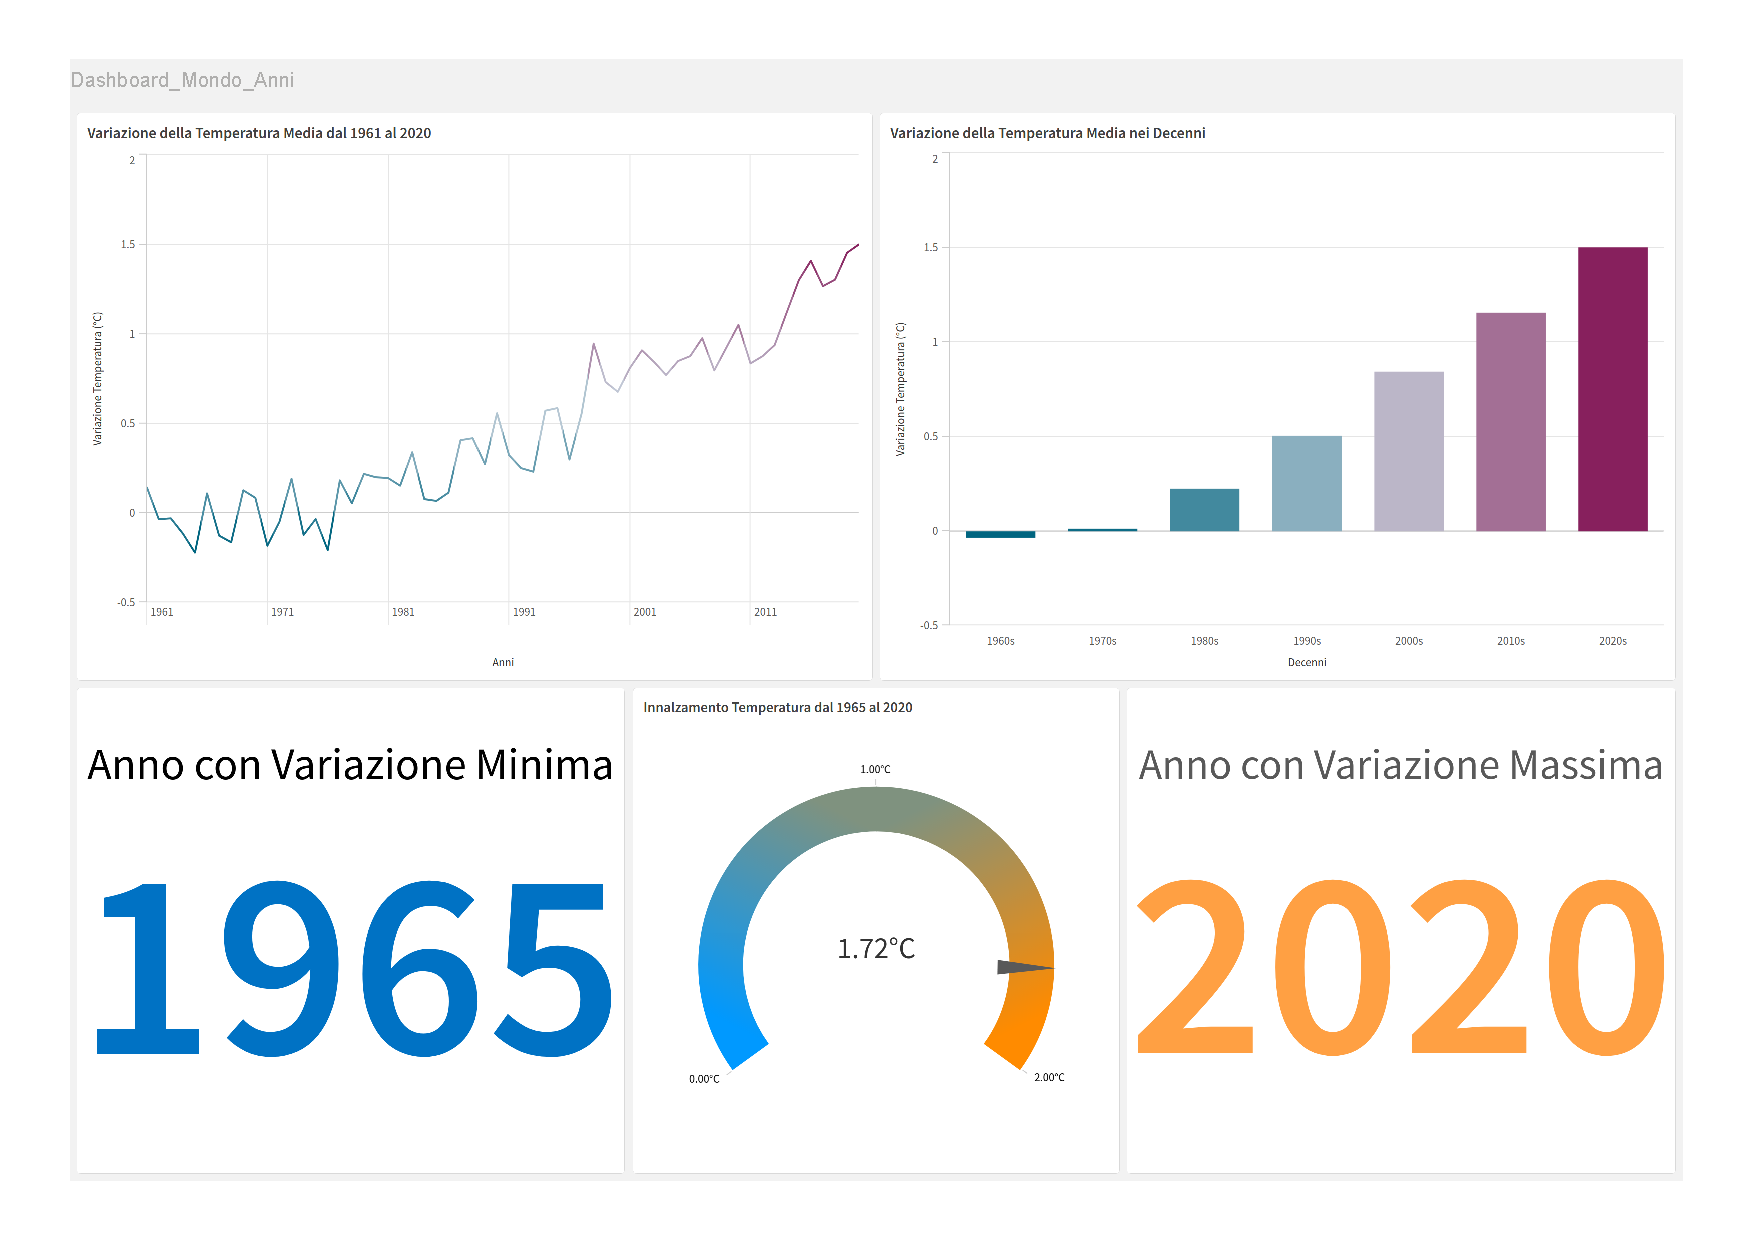
\includegraphics[width=1\linewidth]{capitolo_2/img2/Dashboard_world.pdf}
    \caption{Analisi della variazione della Temperatura Media}
    \label{fig:dashboard_world}
\end{figure}

\subsection{Struttura Dashboard}

\subsection{Filtri applicati}

\begin{comment}
    FARE PROCESSAMENTO DEL DATASET -> UNIONE DATASET
\end{comment}